%%PREAMBLE %%%%%%%%%%%%%%%%%%%%%%%%%%%%
\documentclass[10pt, a4paper]{article}% size of txt = 10pt
\usepackage[top= 2cm,
			bottom = 2cm,
			left = 1.7cm,
			right = 1.7cm,
			footskip = 0.5cm,
			headsep = 0cm,
			headheight = 0cm
					]{geometry}
\usepackage{amsmath} % math packages
\usepackage{amsfonts}% math packages
\usepackage{amssymb} % math packages
\usepackage{graphicx} %package for including graphics
\usepackage{array}
\usepackage[thinlines]{easytable}
\usepackage{float}
\usepackage[section]{placeins}
\usepackage[hidelinks]{hyperref}
\usepackage[shortlabels]{enumitem}
\usepackage{svg}
\usepackage{bigstrut}
\usepackage{wrapfig,lipsum,booktabs}
\usepackage{subcaption}
\usepackage{xfrac}
\usepackage{pdfpages}
\usepackage{listings}
\usepackage{xcolor}


\usepackage{listings}
\usepackage{color} %red, green, blue, yellow, cyan, magenta, black, white
\definecolor{mygreen}{RGB}{28,172,0} % color values Red, Green, Blue
\definecolor{mylilas}{RGB}{170,55,241}

\definecolor{codegreen}{rgb}{0,0.6,0}
\definecolor{codegray}{rgb}{0.5,0.5,0.5}
\definecolor{codepurple}{rgb}{0.58,0,0.82}
\definecolor{backcolour}{rgb}{1,1,1}

\lstdefinestyle{mystyle}{
    backgroundcolor=\color{backcolour},   
    commentstyle=\color{codegreen},
    keywordstyle=\color{magenta},
    numberstyle=\tiny\color{codegray},
    stringstyle=\color{codepurple},
    basicstyle=\ttfamily\footnotesize,
    breakatwhitespace=false,         
    breaklines=true,                 
    captionpos=b,                    
    keepspaces=true,                 
    numbers=left,                    
    numbersep=5pt,                  
    showspaces=false,                
    showstringspaces=false,
    showtabs=false,                  
    tabsize=2
}
\lstset{style=mystyle}


%date format
\def\mydate{\leavevmode\hbox{\twodigits\day.\twodigits\month.\the\year}}
\def\twodigits#1{\ifnum#1<10 0\fi\the#1}

\usepackage{indentfirst}
\setlength{\parindent}{1cm}

\makeatletter
\newcommand{\thickhline}{%
    \noalign {\ifnum 0=`}\fi \hrule height 2pt
    \futurelet \reserved@a \@xhline
}
\newcolumntype{"}{@{\hskip\tabcolsep\vrule width 2pt\hskip\tabcolsep}}
\makeatother
\newcolumntype{?}{!{\vrule width 2pt}}
%%DOC ENVIROMENT%%%%%%%%%%%%%%%%%%%%%%%
\begin{document}
%Title 
\begin{flushleft}%% left justification
	\textbf{\Large{MKC-PKS: Počítačové cvičení}}\hfill Filip Paul\\
	\large{Návrh sítě \hfill\mydate}
	
\end{flushleft}
\section*{Návrh sítě:}
Vygenerovaná síť má následující adresní prostor:
		\begin{figure}[ht!]
			\centering
			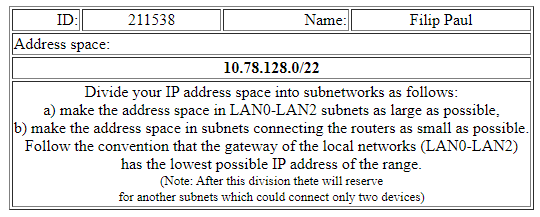
\includegraphics[]{zadani.PNG}
		\end{figure}

Bohužel jsem se podíval na obrázek a rovnou jsem začal vytvářet síť podle postupu, který jsme dělali v prezenčních cvikách,
což tak nějak neodpovídá zadání. Především tomu, že každá podsíť může využít až 31 IP adres. V mojem řešení
je pro routery propojené napřímo dedikovaná menší síť. Celkově vznikne 6 podsítí.
Pro výpočty parametrů sítí jsem využil vlastní python script, který si můžete zobrazit buď v mém GITHUB repozitáři
\href{https://github.com/FilipPaul/ctvrtak_letni_semestr/blob/main/MKC_NSB/ukol1_kryptografie/README.md}{\color{blue} zde} nebo
na konci dokumentu. V github repozitáři taky naleznete cisco\_project.pkt soubor z PC simulace.
		\begin{figure}[ht!]
			\centering
			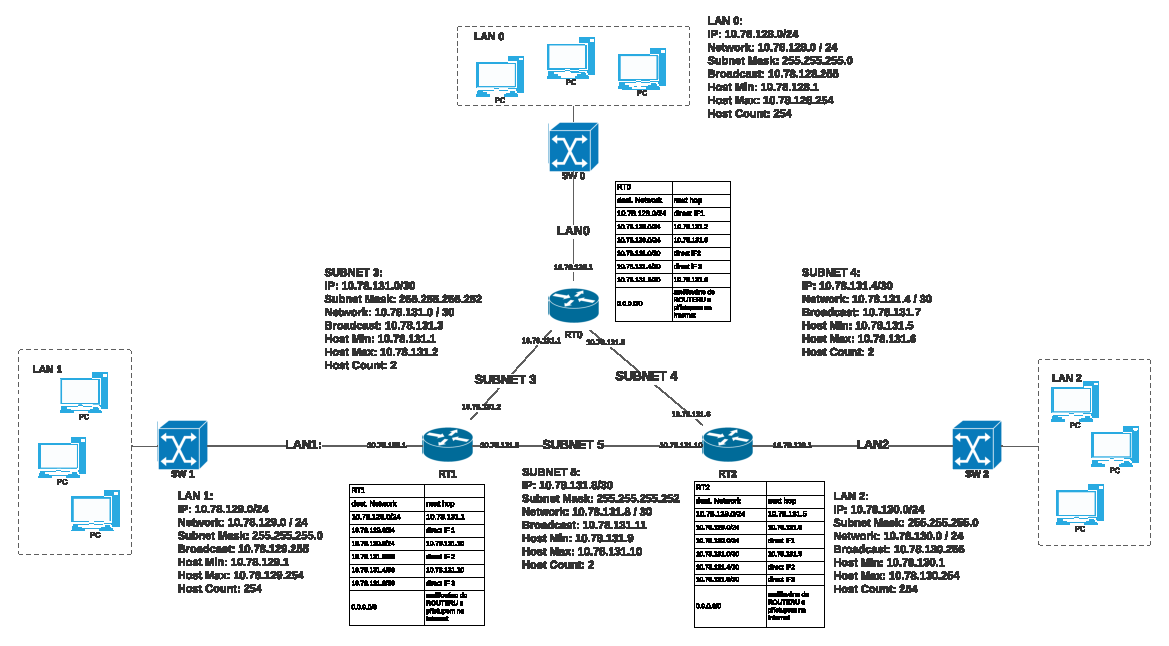
\includegraphics[width = 1\textwidth]{navrhSite.eps}
		\end{figure}	

\section*{PC simulace:}
\begin{figure}[ht!]
    \centering
    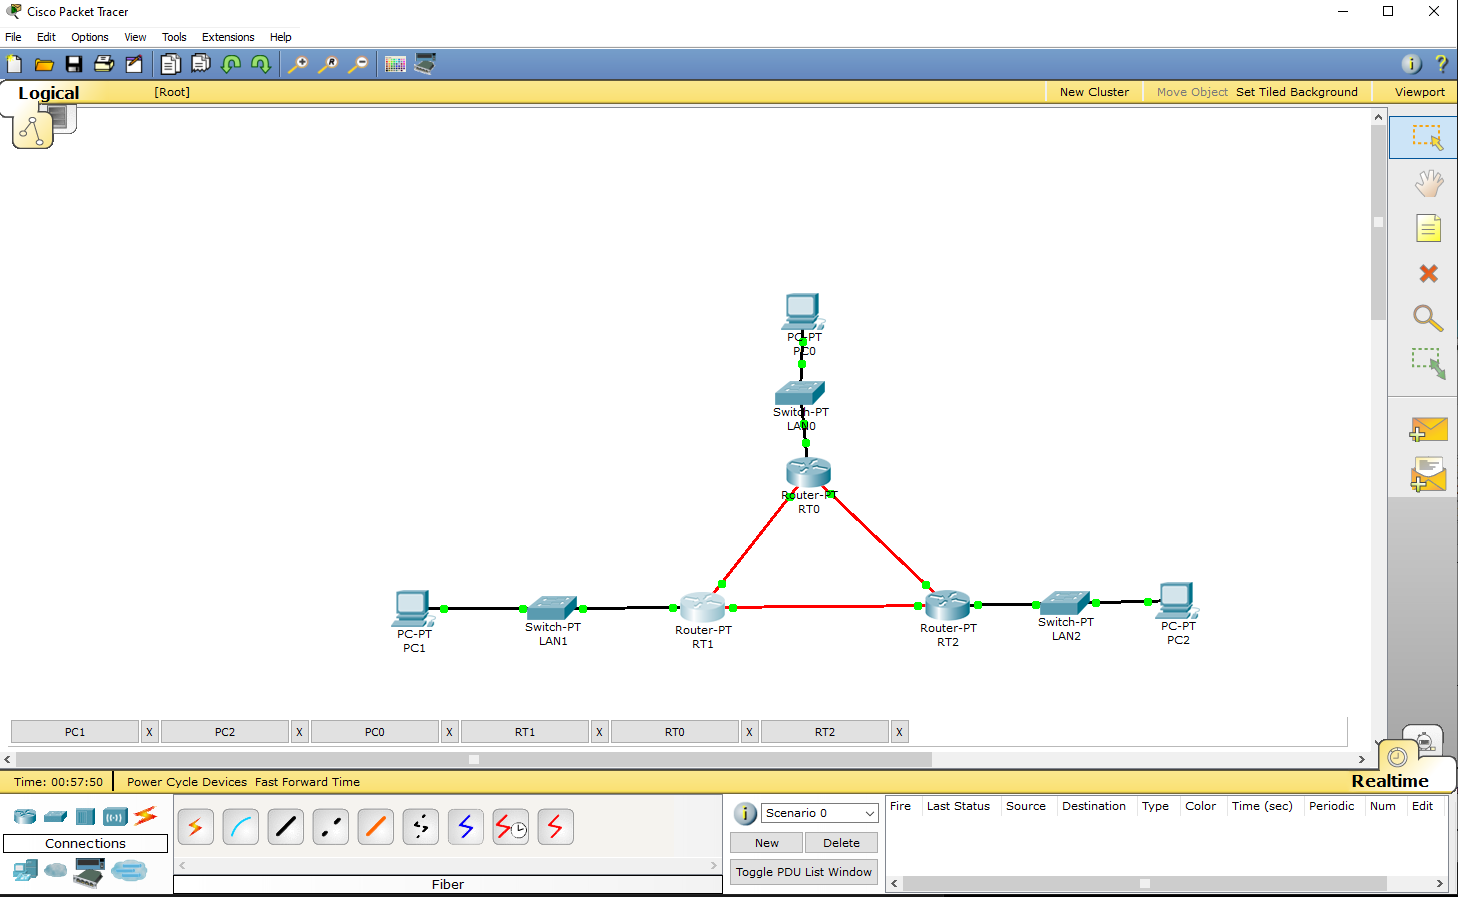
\includegraphics[width = 1\textwidth]{CISCO_diag.PNG}
\end{figure}	

\begin{figure}[ht!]
    \centering
    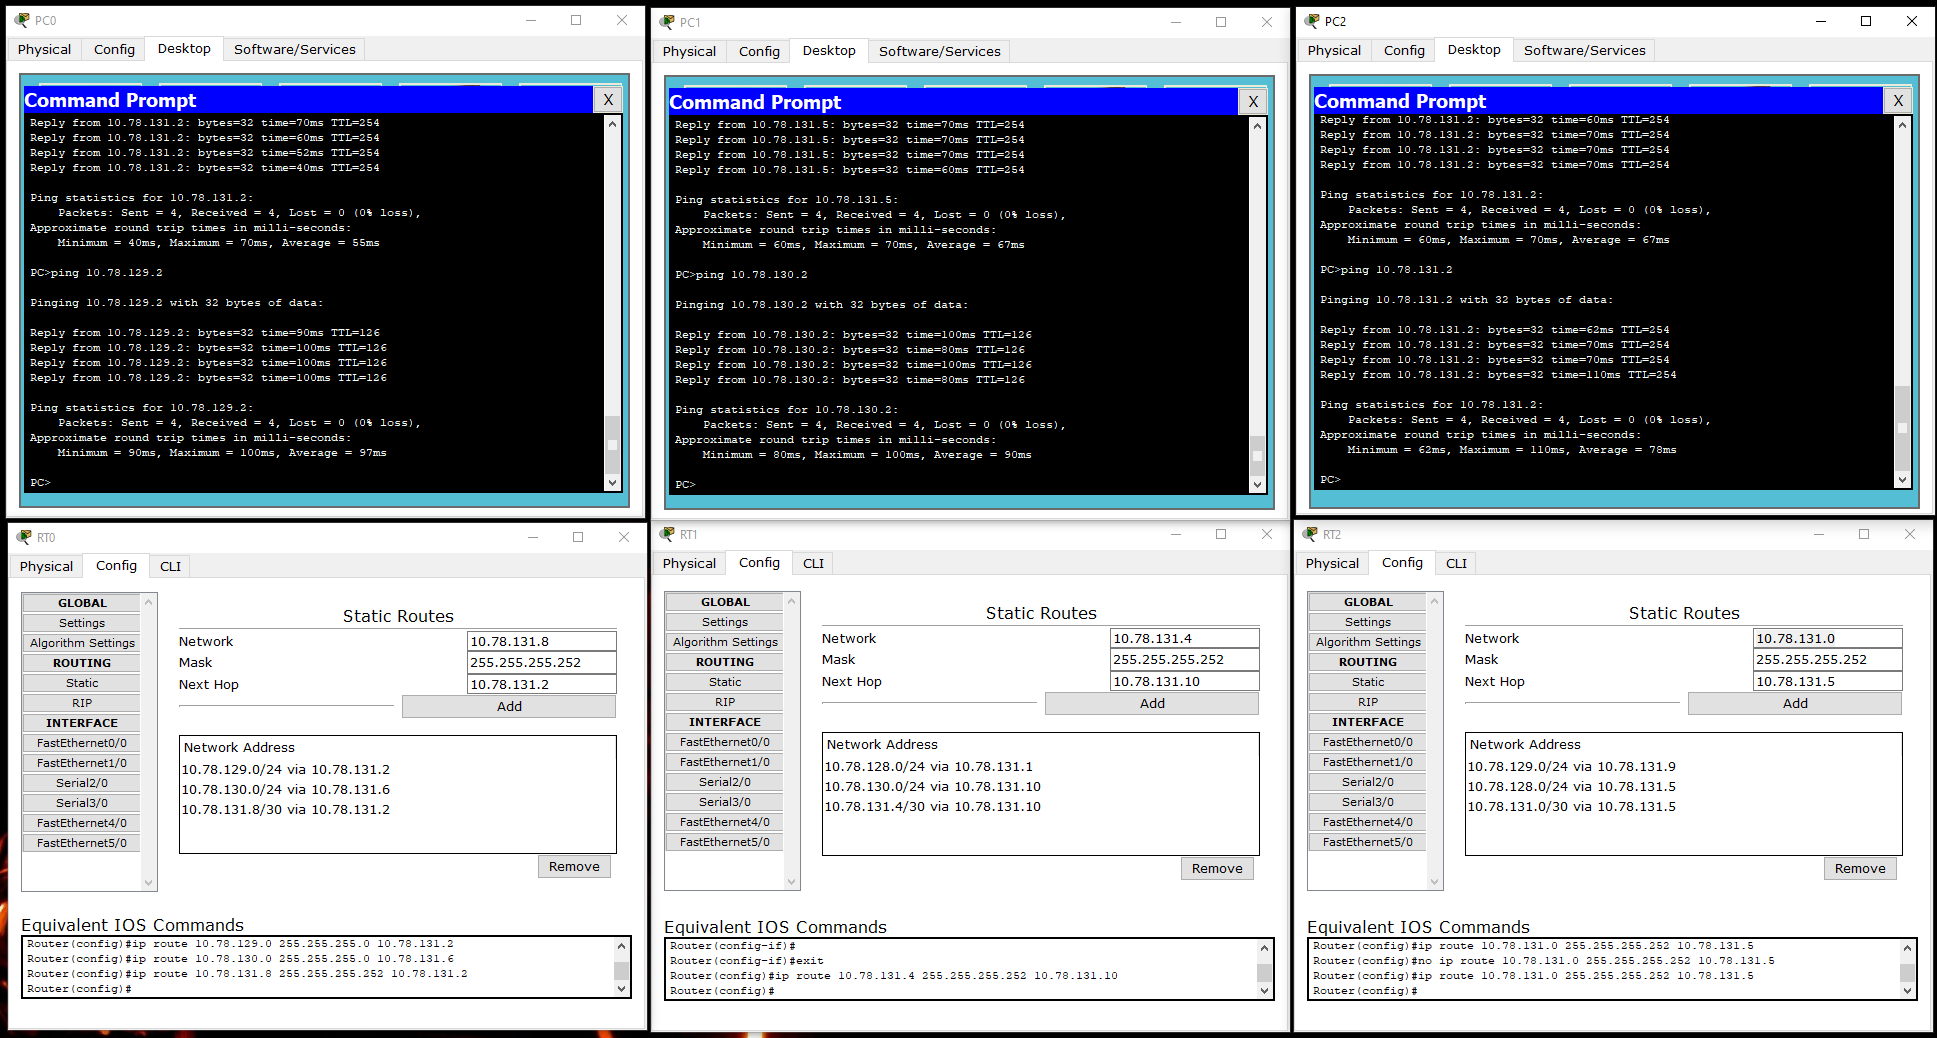
\includegraphics[width = 1\textwidth]{CISCO_config.PNG}
\end{figure}	

\clearpage

\section*{Přílohy:}
\noindent \textbf{calc.py}
\lstinputlisting[language=python]{calc.py}
\textbf{OUTPUT:}
K dispozici:\\
IP Address full format: 10.78.128.0/22\\
IP: 10.78.128.0\\
IP Bits: 00001010.01001110.10000000.00000000\\
Subnet Mask: 255.255.252.0 suffix: 22\\
Subnet Mask Bits: 11111111.11111111.11111100.00000000\\
\\
Network: 10.78.128.0 / 22\\
Broadcast: 10.78.131.255\\
Host Min: 10.78.128.1\\
Host Max: 10.78.131.254\\
Host Count: 1022\\
\\
LAN 0\\
IP Address full format: 10.78.128.0/24\\
IP: 10.78.128.0\\
IP Bits: 00001010.01001110.10000000.00000000\\
Subnet Mask: 255.255.255.0 suffix: 24\\
Subnet Mask Bits: 11111111.11111111.11111111.00000000\\
\\
Network: 10.78.128.0 / 24\\
Broadcast: 10.78.128.255\\
Host Min: 10.78.128.1\\
Host Max: 10.78.128.254\\
Host Count: 254\\
\\
LAN 1\\
IP Address full format: 10.78.129.0/24\\
IP: 10.78.129.0\\
IP Bits: 00001010.01001110.10000001.00000000\\
Subnet Mask: 255.255.255.0 suffix: 24\\
Subnet Mask Bits: 11111111.11111111.11111111.00000000\\
\\
Network: 10.78.129.0 / 24\\
Broadcast: 10.78.129.255\\
Host Min: 10.78.129.1\\
Host Max: 10.78.129.254\\
Host Count: 254\\
\\
LAN 2\\
IP Address full format: 10.78.130.0/24\\
IP: 10.78.130.0\\
IP Bits: 00001010.01001110.10000010.00000000\\
Subnet Mask: 255.255.255.0 suffix: 24\\
Subnet Mask Bits: 11111111.11111111.11111111.00000000\\
\\
Network: 10.78.130.0 / 24\\
Broadcast: 10.78.130.255\\
Host Min: 10.78.130.1\\
Host Max: 10.78.130.254\\
Host Count: 254\\
\\
SUBNET 3\\
IP Address full format: 10.78.131.0/30\\
IP: 10.78.131.0\\
IP Bits: 00001010.01001110.10000011.00000000\\
Subnet Mask: 255.255.255.252 suffix: 30\\
Subnet Mask Bits: 11111111.11111111.11111111.11111100\\
\\
Network: 10.78.131.0 / 30\\
Broadcast: 10.78.131.3\\
Host Min: 10.78.131.1\\
Host Max: 10.78.131.2\\
Host Count: 2\\
\\
SUBNET 4\\
IP Address full format: 10.78.131.4/30\\
IP: 10.78.131.4\\
IP Bits: 00001010.01001110.10000011.00000100\\
Subnet Mask: 255.255.255.252 suffix: 30\\
Subnet Mask Bits: 11111111.11111111.11111111.11111100\\
\\
Network: 10.78.131.4 / 30\\
Broadcast: 10.78.131.7\\
Host Min: 10.78.131.5\\
Host Max: 10.78.131.6\\
Host Count: 2\\
\\
SUBNET 5\\
IP Address full format: 10.78.131.8/30\\
IP: 10.78.131.8\\
IP Bits: 00001010.01001110.10000011.00001000\\
Subnet Mask: 255.255.255.252 suffix: 30\\
Subnet Mask Bits: 11111111.11111111.11111111.11111100\\
\\
Network: 10.78.131.8 / 30\\
Broadcast: 10.78.131.11\\
Host Min: 10.78.131.9\\
Host Max: 10.78.131.10\\
Host Count: 2\\

\noindent  \textbf{myIPAdress.py}
\lstinputlisting[language=python]{myIPAdress.py}
\end{document}